\chapter{Шардинг}

\begin{epigraphs}
\qitem{Если ешь слона, не пытайся запихать его в рот целиком.}{Народная мудрость}
\end{epigraphs}

\section{Введение}

Шардинг~--- разделение данных на уровне ресурсов. Концепция шардинга заключается в логическом разделении данных по различным ресурсам исходя из требований к нагрузке.

Рассмотрим пример. Пусть у нас есть приложение с регистрацией пользователей, которое позволяет писать друг другу личные сообщения. Допустим оно очень популярно и много людей им пользуются ежедневно. Естественно, что таблица с личными сообщениями будет намного больше всех остальных таблиц в базе (скажем, будет занимать 90\% всех ресурсов). Зная это, мы можем подготовить для этой (только одной!) таблицы выделенный сервер помощнее, а остальные оставить на другом (послабее). Теперь мы можем идеально подстроить сервер для работы с одной специфической таблицей, постараться уместить ее в память, возможно, дополнительно партиционировать ее и т.д. Такое распределение называется вертикальным шардингом.

Что делать, если наша таблица с сообщениями стала настолько большой, что даже выделенный сервер под нее одну уже не спасает? Необходимо делать горизонтальный шардинг~--- т.е. разделение одной таблицы по разным ресурсам. Как это выглядит на практике? На разных серверах у нас будет таблица с одинаковой структурой, но разными данными. Для нашего случая с сообщениями, мы можем хранить первые 10 миллионов сообщений на одном сервере, вторые 10 - на втором и т.д. Т.е. необходимо иметь критерий шардинга~--- какой-то параметр, который позволит определять, на каком именно сервере лежат те или иные данные.

Обычно, в качестве параметра шардинга выбирают ID пользователя (\lstinline!user_id!)~--- это позволяет делить данные по серверам равномерно и просто. Т.о. при получении личных сообщений пользователей алгоритм работы будет такой:

\begin{itemize}
  \item Определить, на каком сервере БД лежат сообщения пользователя исходя из \lstinline!user_id!;
  \item Инициализировать соединение с этим сервером;
  \item Выбрать сообщения;
\end{itemize}

Задачу определения конкретного сервера можно решать двумя путями:

\begin{itemize}
  \item Хранить в одном месте хеш-таблицу с соответствиями <<пользователь=сервер>>. Тогда, при определении сервера, нужно будет выбрать сервер из этой таблицы. В этом случае узкое место~--- это большая таблица соответствия, которую нужно хранить в одном месте. Для таких целей очень хорошо подходят базы данных <<ключ=значение>>;
  \item Определять имя сервера с помощью числового (буквенного) преобразования. Например, можно вычислять номер сервера, как остаток от деления на определенное число (количество серверов, между которыми Вы делите таблицу). В этом случае узкое место~--- это проблема добавления новых серверов~--- придется делать перераспределение данных между новым количеством серверов;
\end{itemize}

Естественно, делая горизонтальный шардинг, Вы ограничиваете себя в возможности выборок, которые требуют пересмотра всей таблицы (например, последние посты в блогах людей будет достать невозможно, если таблица постов шардится). Такие задачи придется решать другими подходами. Например, для описанного примера, можно при появлении нового поста, заносить его ID в общий стек, размером в 100 элементом.

Горизонтальный шардинг имеет одно явное преимущество~--- он бесконечно масштабируем. Для создания шардинга PostgreSQL существует несколько решений:

\begin{itemize}
  \item \href{http://postgres-xc.sourceforge.net/}{Postgres-XC}
  \item \href{http://www.greenplum.com/products/greenplum-database}{Greenplum Database}
  \item \href{https://github.com/citusdata/citus}{Citus}
  \item \href{http://plproxy.projects.postgresql.org/doc/tutorial.html}{PL/Proxy}
  \item \href{https://launchpad.net/stado}{Stado (sequel to GridSQL)}
\end{itemize}


\section{PL/Proxy}
\label{sec:plproxy}
PL/Proxy представляет собой прокси-язык для удаленного вызова процедур и партицирования данных между разными базами.
Основная идея его использования заключается в том, что появляется возможность вызывать функции, расположенные в удаленных
базах, а также свободно работать с кластером баз данных (например, вызвать функцию на всех узлах кластера, или на
случайном узле, или на каком-то одном определенном).

Чем PL/Proxy может быть полезен? Он существенно упрощает горизонтальное масштабирование системы.
Становится удобным разделять таблицу с пользователями, например, по первой латинской букве имени~--- на 26 узлов.
При этом приложение, которое работает непосредственно с прокси-базой, ничего не будет замечать: запрос на авторизацию,
например, сам будет направлен прокси-сервером на нужный узел. То есть администратор баз данных может проводить масштабирование
системы практически независимо от разработчиков приложения.

PL/Proxy позволяет полностью решить проблемы масштабирования OLTP систем. В систему легко вводится резервирование с
failover-ом не только по узлам, но и по самим прокси-серверам, каждый из которых работает со всеми узлами.

Недостатки и ограничения:
\begin{itemize}
\item все запросы и вызовы функций вызываются в autocommit-режиме на удаленных серверах
\item в теле функции разрешен только один SELECT; при необходимости нужно писать отдельную процедуру
\item при каждом вызове прокси-сервер стартует новое соединение к бакенд-серверу; в высоконагруженных системах
целесообразно использовать менеджер для кеширования соединений к бакенд-серверам, для этой цели идеально подходит PgBouncer
\item изменение конфигурации кластера (количества партиций, например) требует перезапуска прокси-сервера
\end{itemize}


\subsection{Установка}
\begin{enumerate}
\item Скачать PL/Proxy\footnote{http://pgfoundry.org/projects/plproxy} и распаковать.
\item Собрать PL/Proxy командами make и make install.
\end{enumerate}

Так же можно установить PL/Proxy из репозитория пакетов.
Например в Ubuntu Server достаточно выполнить команду для PostgreSQL 8.4:
\begin{lstlisting}[label=lst:plproxy1,caption=Установка]
sudo aptitude install postgresql-8.4-plproxy
\end{lstlisting}

\subsection{Настройка}
Для примера настройки используется 3 сервера PostgreSQL. 2 сервера пусть будут node1 и node2,
а главный, что будет проксировать запросы на два других~--- proxy.
Для корректной работы pl/proxy рекомендуется использовать количество нод равное степеням двойки.
База данных будет называтся plproxytest, а таблица в ней~--- users. Начнем!

Для начала настроим node1 и node2. Команды написанные ниже нужно выполнять на каждой ноде.

Создадим базу данных plproxytest(если её ещё нет):
\begin{lstlisting}[language=SQL,label=lst:plproxy2,caption=Настройка]
CREATE DATABASE plproxytest
     WITH OWNER = postgres
       ENCODING = 'UTF8';
\end{lstlisting}

Добавляем табличку users:
\begin{lstlisting}[language=SQL,label=lst:plproxy3,caption=Настройка]
CREATE TABLE public.users
  (
   username character varying(255),
   email character varying(255)
  )
  WITH (OIDS=FALSE);
ALTER TABLE public.users OWNER TO postgres;
\end{lstlisting}

Теперь создадим функцию для добавления данных в таблицу users:
\begin{lstlisting}[language=SQL,label=lst:plproxy4,caption=Настройка]
CREATE OR REPLACE FUNCTION public.insert_user(i_username text,
i_emailaddress   text)
RETURNS integer AS
$BODY$
INSERT INTO public.users (username, email) VALUES ($1,$2);
    SELECT 1;
$BODY$
  LANGUAGE 'sql' VOLATILE;
ALTER FUNCTION public.insert_user(text, text) OWNER TO postgres;
\end{lstlisting}

С настройкой нодов закончено. Приступим к серверу proxy.

Как и на всех нодах, на главном сервере (proxy) должна присутствовать база данных:
\begin{lstlisting}[language=SQL,label=lst:plproxy5,caption=Настройка]
CREATE DATABASE plproxytest
     WITH OWNER = postgres
       ENCODING = 'UTF8';
\end{lstlisting}

Теперь надо указать серверу что эта база данных управляется с помощью pl/proxy:
\begin{lstlisting}[language=SQL,label=lst:plproxy6,caption=Настройка]
CREATE OR REPLACE FUNCTION public.plproxy_call_handler()
  RETURNS language_handler AS
'$libdir/plproxy', 'plproxy_call_handler'
  LANGUAGE 'c' VOLATILE
COST 1;
ALTER FUNCTION public.plproxy_call_handler()
OWNER TO postgres;
-- language
CREATE LANGUAGE plproxy HANDLER plproxy_call_handler;
CREATE LANGUAGE plpgsql;
\end{lstlisting}

Также, для того что бы сервер знал где и какие ноды у него есть, надо создать 3 сервисные функции, которые pl/proxy будет использовать в своей работе. Первая функция~--- конфиг для кластера баз данных. Тут указываются параметры через key-value:
\begin{lstlisting}[language=SQL,label=lst:plproxy7,caption=Настройка]
CREATE OR REPLACE FUNCTION public.get_cluster_config
(IN cluster_name text,   OUT "key" text, OUT val text)
  RETURNS SETOF record AS
$BODY$
BEGIN
  -- lets use same config for all clusters
  key := 'connection_lifetime';
  val := 30*60; -- 30m
  RETURN NEXT;
  RETURN;
END;
$BODY$
  LANGUAGE 'plpgsql' VOLATILE
  COST 100
  ROWS 1000;
ALTER FUNCTION public.get_cluster_config(text)
OWNER TO postgres;
\end{lstlisting}

Вторая важная функция, код которой надо будет подправить. В ней надо будет указать DSN нод:
\begin{lstlisting}[language=SQL,label=lst:plproxy8,caption=Настройка]
CREATE OR REPLACE FUNCTION
public.get_cluster_partitions(cluster_name text)
  RETURNS SETOF text AS
$BODY$
BEGIN
  IF cluster_name = 'usercluster' THEN
    RETURN NEXT 'dbname=plproxytest host=node1 user=postgres';
    RETURN NEXT 'dbname=plproxytest host=node2 user=postgres';
    RETURN;
  END IF;
  RAISE EXCEPTION 'Unknown cluster';
END;
$BODY$
  LANGUAGE 'plpgsql' VOLATILE
  COST 100
  ROWS 1000;
ALTER FUNCTION public.get_cluster_partitions(text)
OWNER TO postgres;
\end{lstlisting}

И последняя:
\begin{lstlisting}[language=SQL,label=lst:plproxy9,caption=Настройка]
CREATE OR REPLACE FUNCTION
public.get_cluster_version(cluster_name text)
  RETURNS integer AS
$BODY$
BEGIN
  IF cluster_name = 'usercluster' THEN
    RETURN 1;
  END IF;
  RAISE EXCEPTION 'Unknown cluster';
END;
$BODY$
  LANGUAGE 'plpgsql' VOLATILE
  COST 100;
ALTER FUNCTION public.get_cluster_version(text)
OWNER TO postgres;
\end{lstlisting}

Ну и собственно самая главная функция, которая будет вызываться уже непосредственно в приложении:
\begin{lstlisting}[language=SQL,label=lst:plproxy10,caption=Настройка]
CREATE OR REPLACE FUNCTION
public.insert_user(i_username text, i_emailaddress text)
  RETURNS integer AS
$BODY$
  CLUSTER 'usercluster';
  RUN ON hashtext(i_username);
$BODY$
  LANGUAGE 'plproxy' VOLATILE
  COST 100;
ALTER FUNCTION public.insert_user(text, text)
OWNER TO postgres;
\end{lstlisting}

Все готово. Подключаемся к серверу proxy и заносим данные в базу:
\begin{lstlisting}[language=SQL,label=lst:plproxy11,caption=Настройка]
SELECT insert_user('Sven','sven@somewhere.com');
SELECT insert_user('Marko', 'marko@somewhere.com');
SELECT insert_user('Steve','steve@somewhere.com');
\end{lstlisting}

Пробуем извлечь данные.
Для этого напишем новую серверную функцию:
\begin{lstlisting}[language=SQL,label=lst:plproxy12,caption=Настройка]
CREATE OR REPLACE FUNCTION
public.get_user_email(i_username text)
 RETURNS SETOF text AS
$BODY$
 CLUSTER 'usercluster';
 RUN ON hashtext(i_username) ;
 SELECT email FROM public.users
 WHERE username = i_username;
$BODY$
 LANGUAGE 'plproxy' VOLATILE
 COST 100
 ROWS 1000;
ALTER FUNCTION public.get_user_email(text)
OWNER TO postgres;
\end{lstlisting}

И попробуем её вызвать:
\begin{lstlisting}[language=SQL,label=lst:plproxy13,caption=Настройка]
select plproxy.get_user_email('Steve');
\end{lstlisting}

Если потом подключиться к каждой ноде отдельно, то можно четко увидеть, что данные users разбросаны по таблицам каждой ноды.

\subsection{Все ли так просто?}
Как видно на тестовом примере ничего сложного в работе с pl/proxy нет.
Но, я думаю все кто смог дочитать до этой строчки уже поняли что в реальной жизни все не так просто.
Представьте что у вас 16 нод. Это же надо как-то синхронизировать код функций. А что если ошибка закрадётся~---
как её оперативно исправлять?

Этот вопрос был задан и на конференции Highload++ 2008, на что Аско Ойя ответил что соответствующие средства
уже реализованы внутри самого Skype, но ещё не достаточно готовы для того что бы отдавать их на суд сообществу opensource.

Второй проблема, которая не дай бог коснётся вас при разработке такого рода системы, это проблема перераспределения данных
в тот момент когда нам захочется добавить ещё нод в кластер.
Планировать эту масштабную операцию придётся очень тщательно, подготовив все сервера заранее,
занеся данные и потом в один момент подменив код функции get\_cluster\_partitions.
\section{Citus}
\label{sec:citus}

TODO
\section{Postgres-XC}
\label{sec:postgres-xc}

Postgres-XC~-- система для создания мульти-мастер кластеров, работающих в синхронном режиме~-- все узлы всегда содержат актуальные данные. Postgres-XC поддерживает опции для увеличения масштабирования кластера как при преобладании операций записи, так и при основной нагрузке на чтение данных: поддерживается выполнение транзакций с распараллеливанием на несколько узлов, за целостностью транзакций в пределах всего кластера отвечает специальный узел GTM (Global Transaction Manager).

Измерение производительности показало, что КПД кластера Postgres-XC составляет примерно 64\%, т.е. кластер из 10 серверов позволяет добиться увеличения производительности системы в целом в 6.4 раза, относительно производительности одного сервера (цифры приблизительные).

Система не использует в своей работе триггеры и представляет собой набор дополнений и патчей к PostgreSQL, дающих возможность в прозрачном режиме обеспечить работу в кластере стандартных приложений, без их дополнительной модификации и адаптации (полная совместимость с PostgreSQL API). Кластер состоит из одного управляющего узла (GTM), предоставляющего информацию о состоянии транзакций, и произвольного набора рабочих узлов, каждый из которых в свою очередь состоит из координатора и обработчика данных (обычно эти элементы реализуются на одном сервере, но могут быть и разделены).

Хоть Postgres-XC и выглядит похожим на MultiMaster, но он им не является. Все сервера кластера должны быть соединены сетью с минимальными задержками, никакое географически-распределенное решение с разумной производительностью построить на нем невозможно (это важный момент).

\subsection{Архитектура}

\begin{figure}[ht!]
  \center{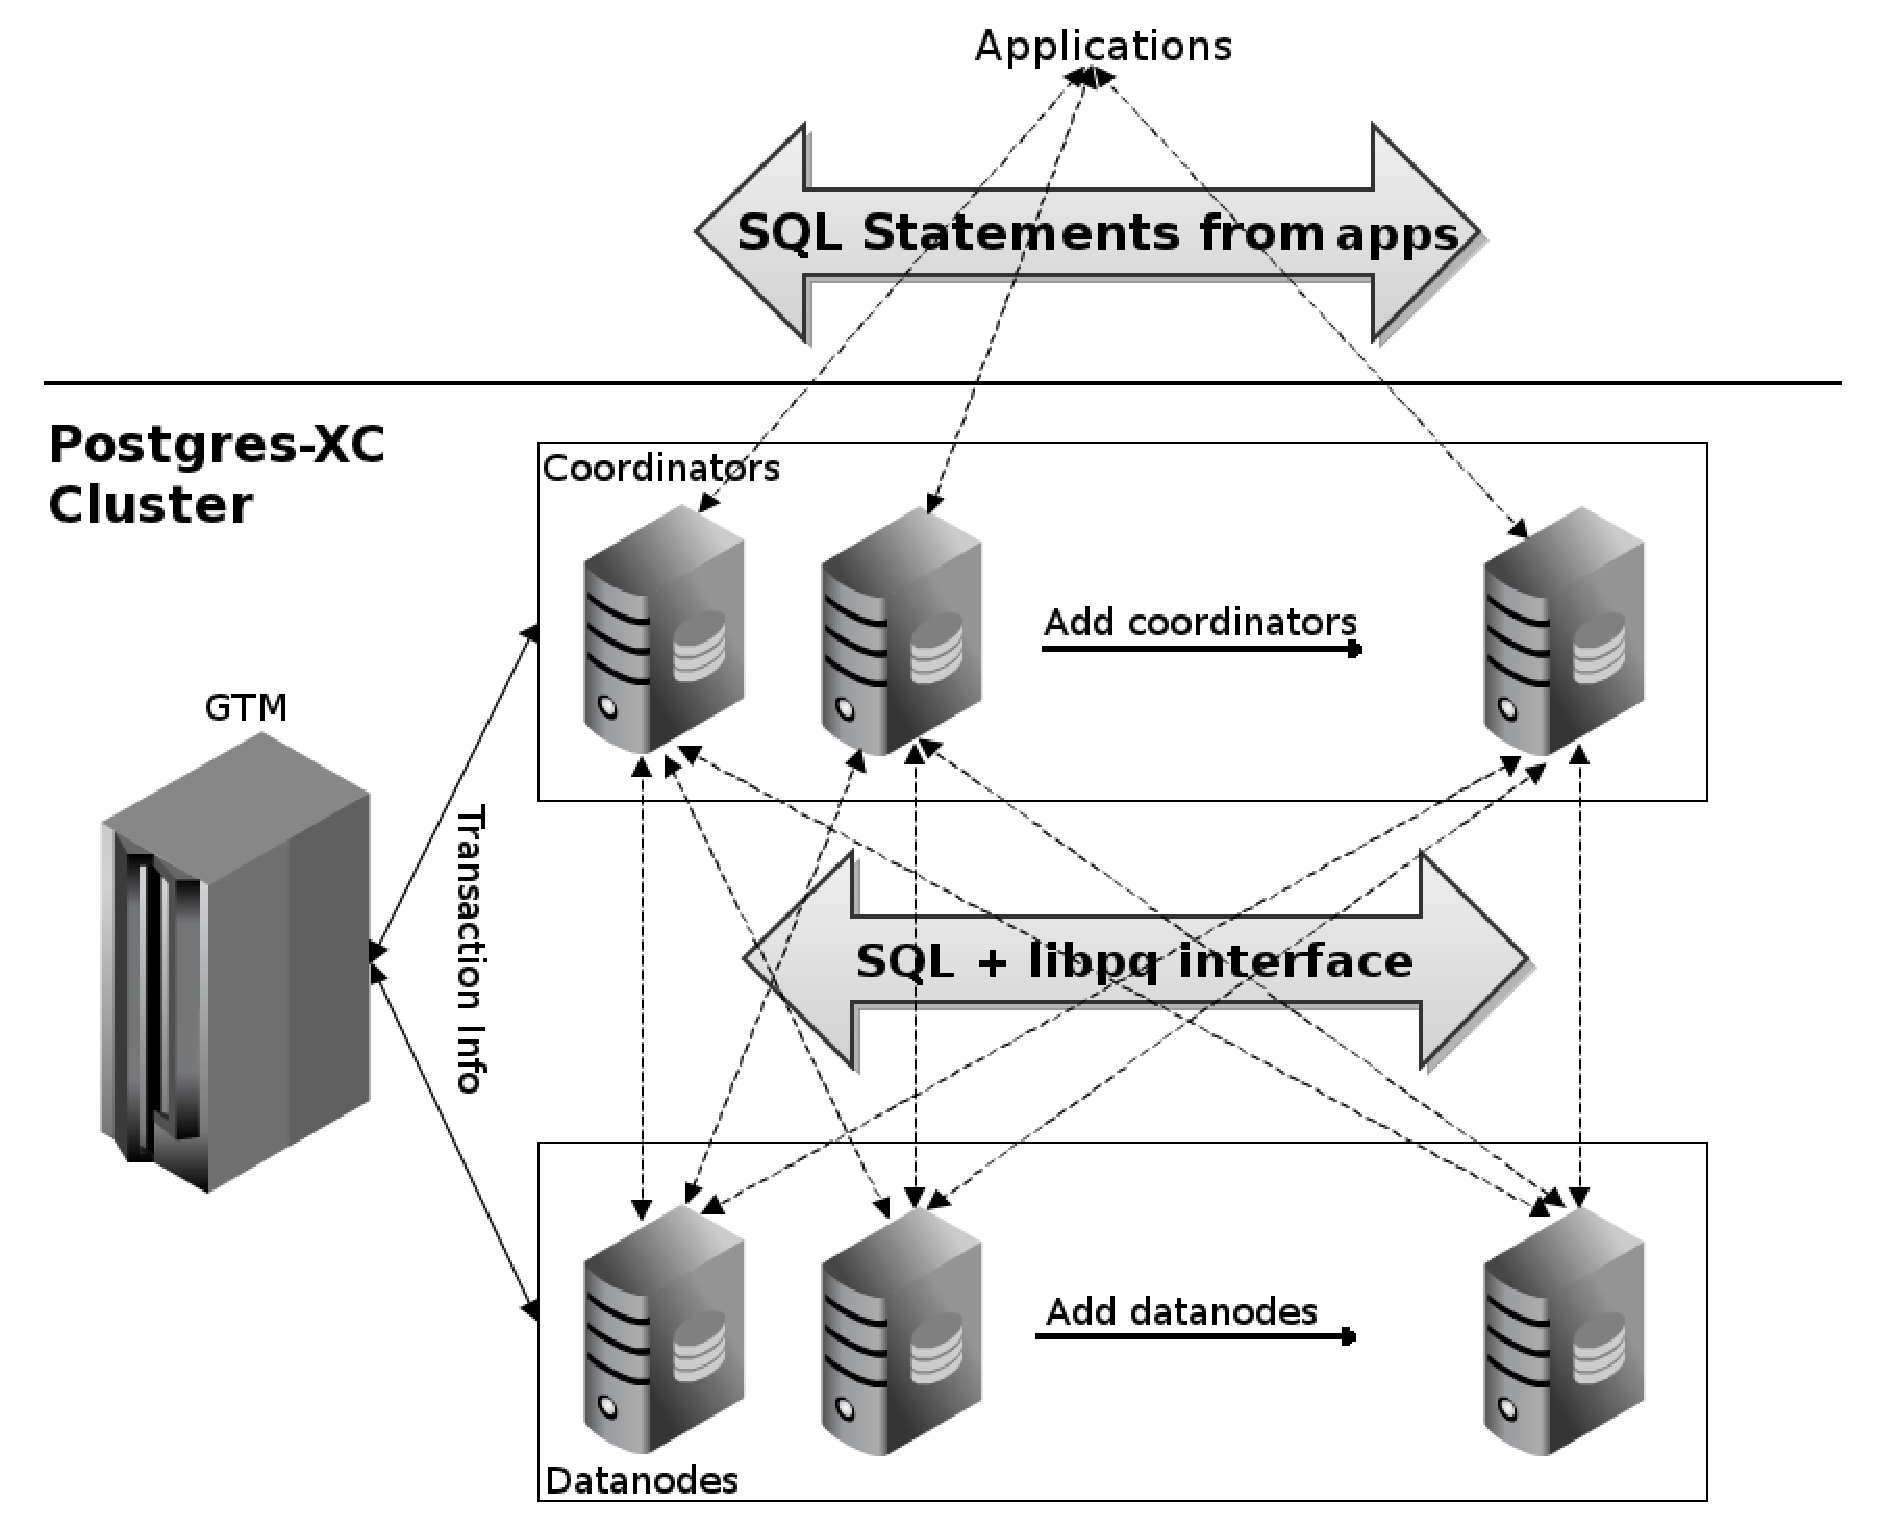
\includegraphics[width=1\textwidth]{postgres-xc-arch.pdf}}
  \caption{Архитектура Postgres-XC}
  \label{fig:postgres-xc1}
\end{figure}

Рис.~\ref{fig:postgres-xc1} показывает архитектуру Postgres-XC с тремя её основными компонентами:

\begin{enumerate}
  \item Глобальный менеджер транзакций (GTM)~--- собирает и обрабатывает информацию о транзакциях в Postgres-XC, решает вопросы глобального идентификатора транзакции по операциям (для поддержания согласованного представления базы данных на всех узлах). Он обеспечивает поддержку других глобальных данных, таких как последовательности и временные метки. Он хранит данные пользователя, за исключением управляющей информации.
  \item Координаторы (coordinators)~--- обеспечивают точку подключения для клиента (приложения). Они несут ответственность за разбор и выполнение запросов от клиентов и возвращение результатов (при необходимости). Они не хранят пользовательские данные, а собирают их из обработчиков данных (datanodes) с помощью запросов SQL через PostgreSQL интерфейс. Координаторы также обрабатывают данные, если требуется, и даже управляют двухфазной фиксацией. Координаторы используются также для разбора запросов, составления планов запросов, поиска данных и т.д.
  \item Обработчики данных (datanodes)~--- обеспечивают сохранение пользовательских данных. Datanodes выполняют запросы от координаторов и возвращают им полученный результат.
\end{enumerate}

\subsection{Установка}

Установить Postgres-XC можно из \href{http://postgres-x2.github.io/}{исходников} или же из пакетов системы. Например в Ubuntu 14.04 можно установить postgres-xc так:

\begin{lstlisting}[language=Bash,label=lst:postgres-xc1,caption=Установка Postgres-XC]
$ sudo apt-get install postgres-xc postgres-xc-client postgres-xc-contrib postgres-xc-server-dev
\end{lstlisting}

По умолчанию он создаст один координатор и два обработчика данных.

\subsection{Распределение данных и масштабируемость}

Postgres-XC предусматривает два способа хранения данных в таблицах:

\begin{figure}[ht!]
  \center{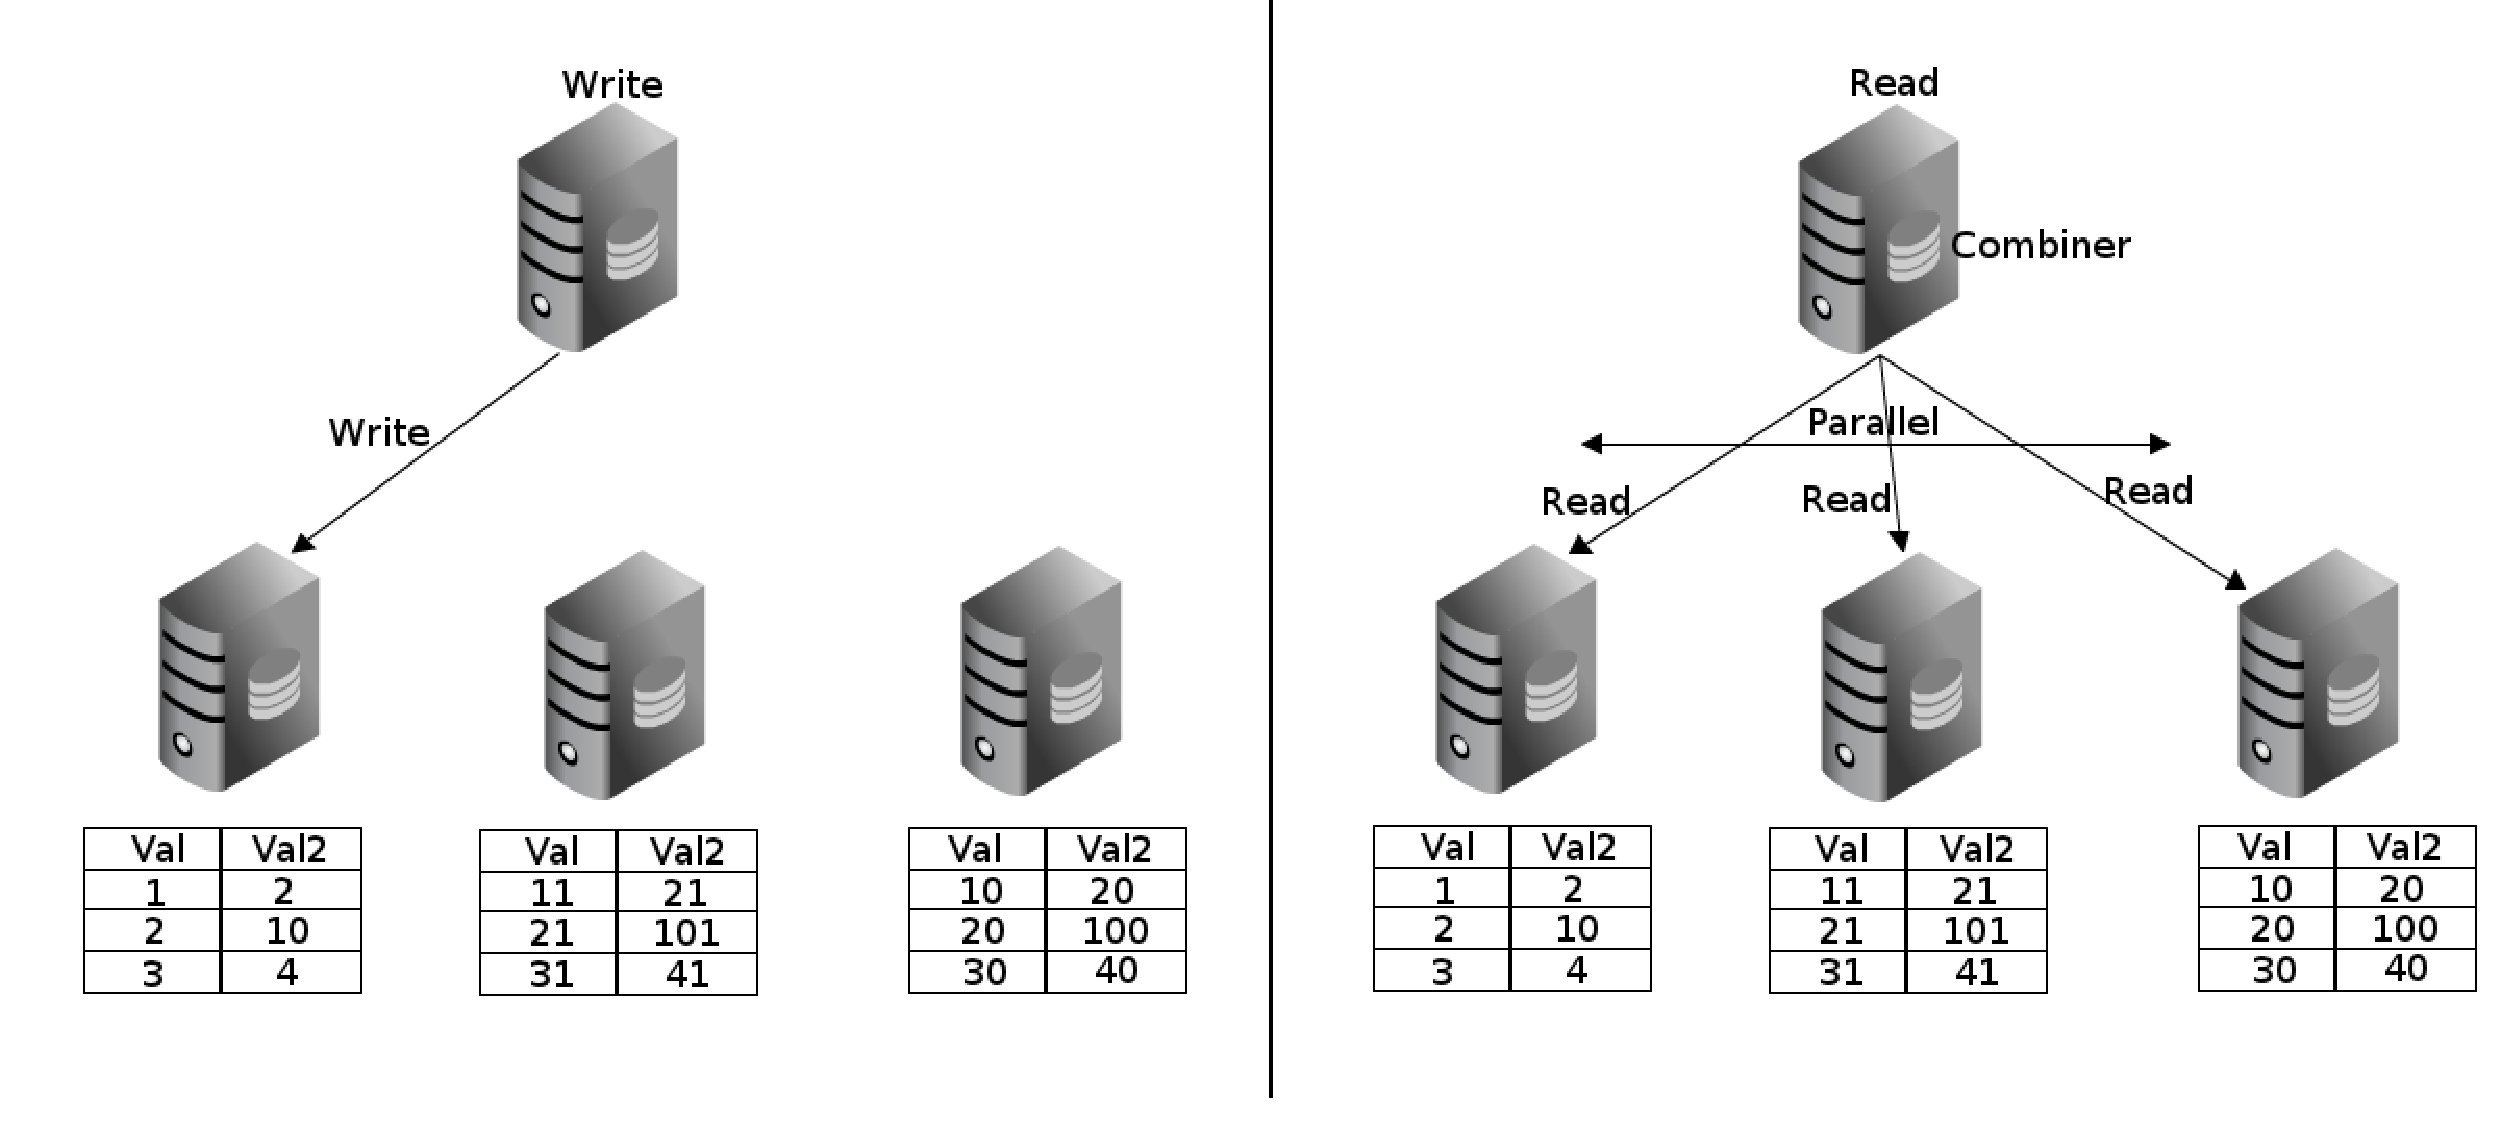
\includegraphics[width=1\textwidth]{postgres-xc-02.pdf}}
  \caption{Распределенные таблицы}
  \label{fig:postgres-xc2}
\end{figure}

\begin{figure}[ht!]
  \center{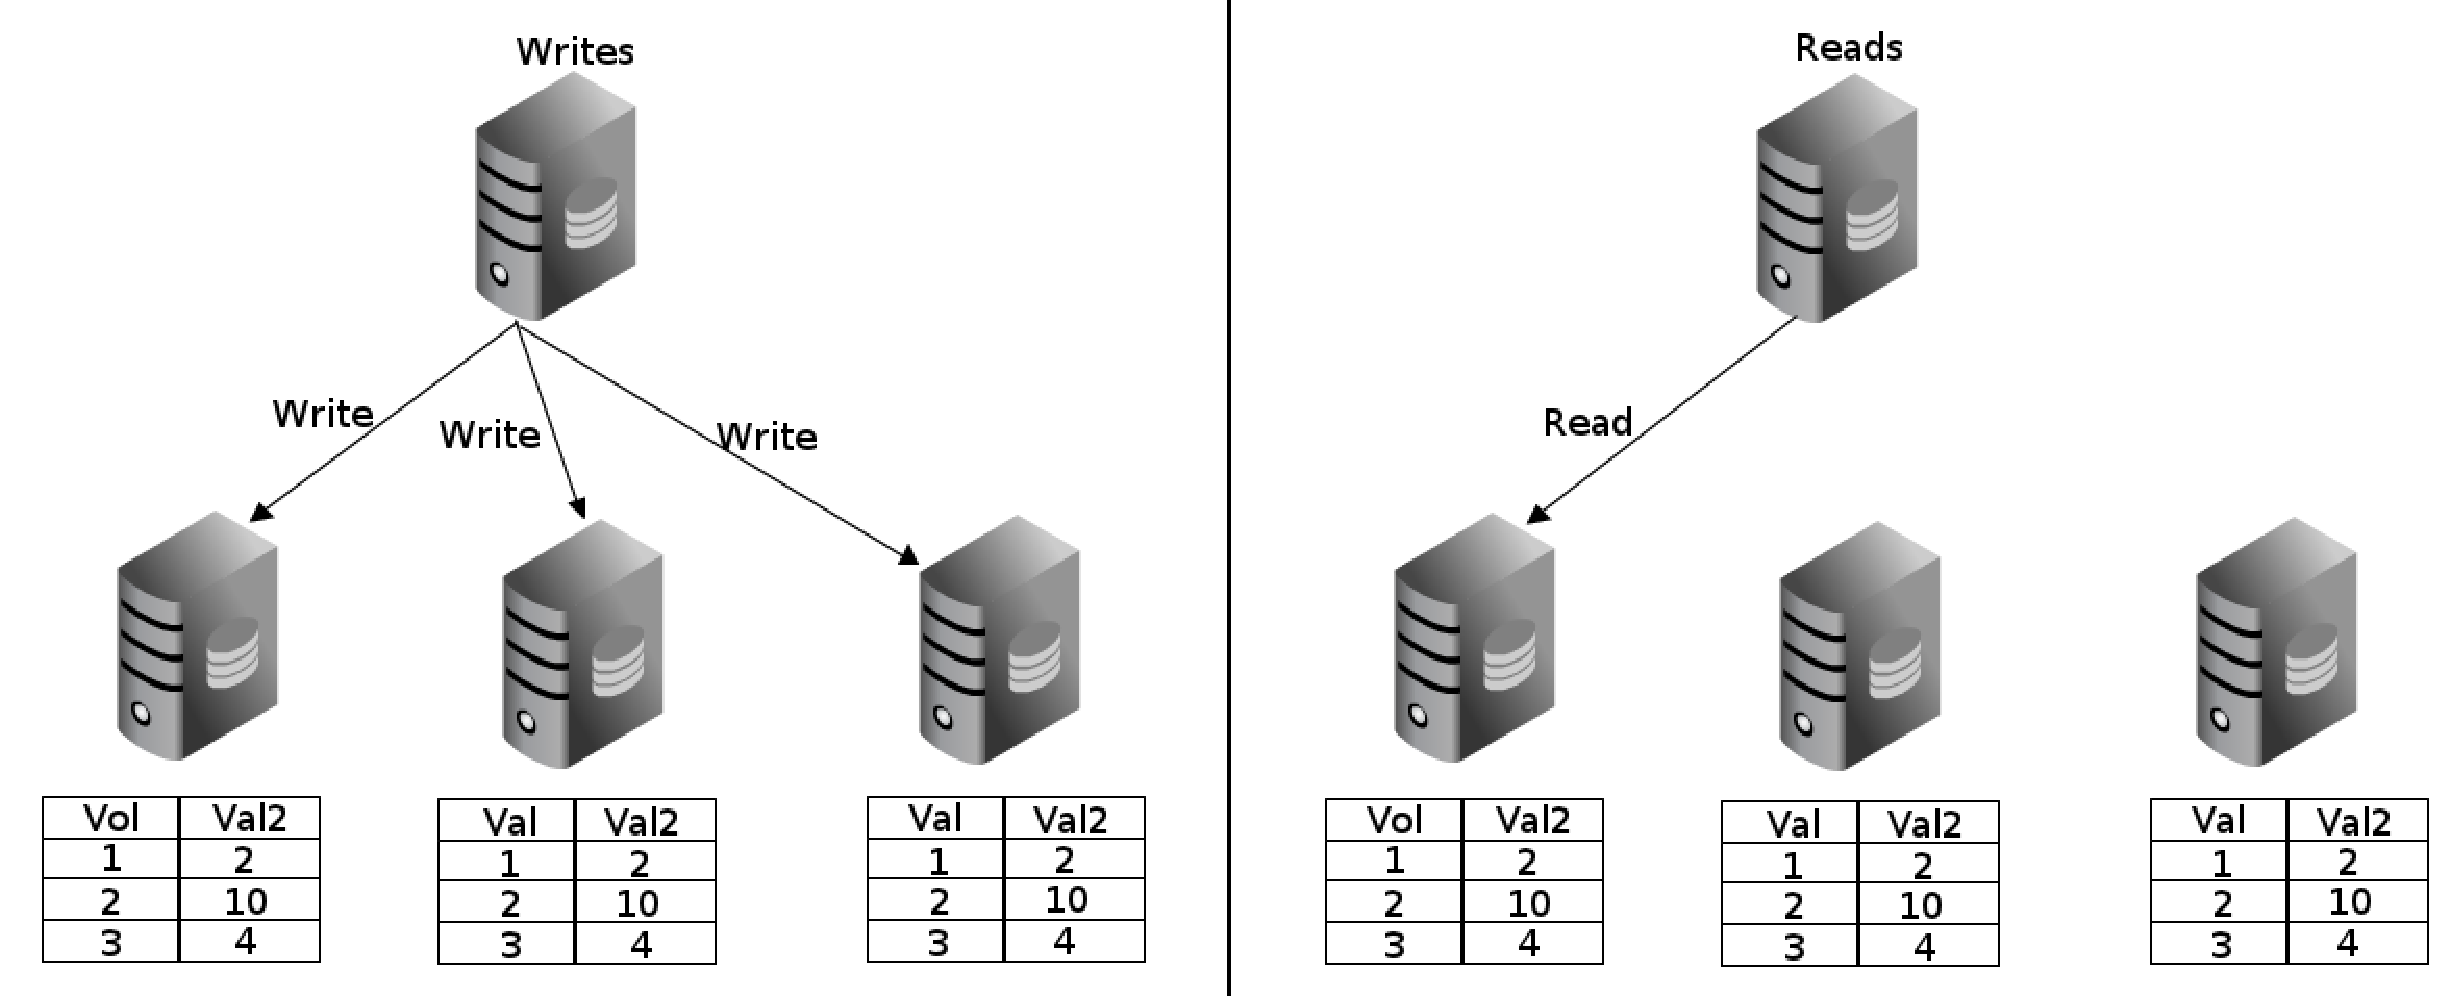
\includegraphics[width=1\textwidth]{postgres-xc-03.pdf}}
  \caption{Реплицированные таблицы}
  \label{fig:postgres-xc3}
\end{figure}

\begin{enumerate}
  \item Распределенные таблицы (distributed tables, рис.~\ref{fig:postgres-xc2}): данные по таблице распределяются на указанный набор обработчиков данных с использованием указанной стратегии (hash, round-robin, modulo). Каждая запись в таблице находится только на одном обработчике данных. Параллельно могут быть записаны или прочитаны данные с различных обработчиков данных. За счет этого значительно улучшена производительность на запись и чтение;
  \item Реплицированные таблицы (replicated tables, рис.~\ref{fig:postgres-xc3}): данные по таблице реплицируется (клонируются) на указанный набор обработчиков данных. Каждая запись в таблице находится на всех обработчиках данных (которые были указаны) и любые изменения дублируются на все обработчики данных. Так как все данные доступны на любом обработчике данных, координатор может собрать все данные из одного узла, что позволяет направить различные запросы на различные обработчики данных. Таким образом создается балансировка нагрузки и увеличения пропускной способности на чтение.
\end{enumerate}

\subsection{Таблицы и запросы к ним}

После установки работа с Postgres-XC ведется как с обыкновенным PostgreSQL. Подключаться для работы с данными нужно только к координаторам (по умолчанию координатор работает на порту 5432). Для начала создадим распределенные таблицы.

\begin{lstlisting}[language=SQL,label=lst:postgres-xc2,caption=Создание распределенных таблиц]
CREATE TABLE
users_with_hash (id SERIAL, type INT, ...)
DISTRIBUTE by HASH(id);

CREATE TABLE
users_with_modulo (id SERIAL, type INT, ...)
DISTRIBUTE by MODULO(id);

CREATE TABLE
users_with_rrobin (id SERIAL, type INT, ...)
DISTRIBUTE by ROUNDROBIN;
\end{lstlisting}

На листинге~\ref{lst:postgres-xc2} создано 3 распределенные таблицы:

\begin{enumerate}
  \item Таблица \lstinline!users_with_hash! распределяется по хешу значения из указанного поля в таблице (тут указано поле id) по обработчикам данных. Вот как распределились первые 15 значений:

\begin{lstlisting}[language=SQL,label=lst:postgres-xc3,caption=Данные с координатора и обработчиков данных]
# координатор
$ psql
# SELECT id, type from users_with_hash ORDER BY id;
 id   | type
-------+-------
     1 |   946
     2 |   153
     3 |   484
     4 |   422
     5 |   785
     6 |   906
     7 |   973
     8 |   699
     9 |   434
    10 |   986
    11 |   135
    12 |  1012
    13 |   395
    14 |   667
    15 |   324

# первый обработчик данных
$ psql -p15432
# SELECT id, type from users_with_hash ORDER BY id;
  id  | type
------+-------
    1 |   946
    2 |   153
    5 |   785
    6 |   906
    8 |   699
    9 |   434
   12 |  1012
   13 |   395
   15 |   324

# второй обработчик данных
$ psql -p15433
# SELECT id, type from users_with_hash ORDER BY id;
 id   | type
-------+-------
     3 |   484
     4 |   422
     7 |   973
    10 |   986
    11 |   135
    14 |   667
\end{lstlisting}

  \item Таблица \lstinline!users_with_modulo! распределяется по модулю значения из указанного поля в таблице (тут указано поле id) по обработчикам данных. Вот как распределились первые 15 значений:

\begin{lstlisting}[language=SQL,label=lst:postgres-xc4,caption=Данные с координатора и обработчиков данных]
# координатор
$ psql
# SELECT id, type from users_with_modulo ORDER BY id;
 id   | type
-------+-------
     1 |   883
     2 |   719
     3 |    29
     4 |   638
     5 |   363
     6 |   946
     7 |   440
     8 |   331
     9 |   884
    10 |   199
    11 |    78
    12 |   791
    13 |   345
    14 |   476
    15 |   860

# первый обработчик данных
$ psql -p15432
# SELECT id, type from users_with_modulo ORDER BY id;
  id   | type
-------+-------
     2 |   719
     4 |   638
     6 |   946
     8 |   331
    10 |   199
    12 |   791
    14 |   476

# второй обработчик данных
$ psql -p15433
# SELECT id, type from users_with_modulo ORDER BY id;
  id  | type
------+-------
    1 |   883
    3 |    29
    5 |   363
    7 |   440
    9 |   884
   11 |    78
   13 |   345
   15 |   860
\end{lstlisting}

  \item Таблица \lstinline!users_with_rrobin! распределяется циклическим способом(round-robin) по обработчикам данных. Вот как распределились первые 15 значений:

\begin{lstlisting}[language=SQL,label=lst:postgres-xc5,caption=Данные с координатора и обработчиков данных]
# координатор
$ psql
# SELECT id, type from users_with_rrobin ORDER BY id;
 id   | type
-------+-------
     1 |   890
     2 |   198
     3 |   815
     4 |   446
     5 |    61
     6 |   337
     7 |   948
     8 |   446
     9 |   796
    10 |   422
    11 |   242
    12 |   795
    13 |   314
    14 |   240
    15 |   733

# первый обработчик данных
$ psql -p15432
# SELECT id, type from users_with_rrobin ORDER BY id;
  id   | type
-------+-------
     2 |   198
     4 |   446
     6 |   337
     8 |   446
    10 |   422
    12 |   795
    14 |   240

# второй обработчик данных
$ psql -p15433
# SELECT id, type from users_with_rrobin ORDER BY id;
  id  | type
------+-------
    1 |   890
    3 |   815
    5 |    61
    7 |   948
    9 |   796
   11 |   242
   13 |   314
   15 |   733
\end{lstlisting}

\end{enumerate}

Теперь создадим реплицированную таблицу:

\begin{lstlisting}[language=SQL,label=lst:postgres-xc20,caption=Создание реплицированной таблицы]
CREATE TABLE
users_replicated (id SERIAL, type INT, ...)
DISTRIBUTE by REPLICATION;
\end{lstlisting}

Естественно данные идентичны на всех обработчиках данных:

\begin{lstlisting}[language=SQL,label=lst:postgres-xc21,caption=Данные с координатора и обработчиков данных]
# SELECT id, type from users_replicated  ORDER BY id;
  id   | type
-------+-------
     1 |    75
     2 |   262
     3 |   458
     4 |   779
     5 |   357
     6 |    51
     7 |   249
     8 |   444
     9 |   890
    10 |   810
    11 |   809
    12 |   166
    13 |   605
    14 |   401
    15 |    58
\end{lstlisting}

Рассмотрим как выполняются запросы для таблиц. Выберем все записи из распределенной таблицы:

\begin{lstlisting}[language=SQL,label=lst:postgres-xc6,caption=Выборка записей из распределенной таблицы]
# EXPLAIN VERBOSE SELECT * from users_with_modulo ORDER BY id;
                                      QUERY PLAN
--------------------------------------------------------------------------------------
 Sort  (cost=49.83..52.33 rows=1000 width=8)
   Output: id, type
   Sort Key: users_with_modulo.id
   ->  Result  (cost=0.00..0.00 rows=1000 width=8)
         Output: id, type
         ->  Data Node Scan on users_with_modulo  (cost=0.00..0.00 rows=1000 width=8)
               Output: id, type
               Node/s: dn1, dn2
               Remote query: SELECT id, type FROM ONLY users_with_modulo WHERE true
(9 rows)
\end{lstlisting}

Как видно на листинге~\ref{lst:postgres-xc6} координатор собирает данные из обработчиков данных, а потом собирает их вместе.

Подсчет суммы с группировкой по полю из распределенной таблицы:

\begin{lstlisting}[language=SQL,label=lst:postgres-xc7,caption=Выборка записей из распределенной таблицы]
# EXPLAIN VERBOSE SELECT sum(id) from users_with_modulo GROUP BY type;
                                                                      QUERY PLAN
------------------------------------------------------------------------------------------------------------------------------------------------------
 HashAggregate  (cost=5.00..5.01 rows=1 width=8)
   Output: pg_catalog.sum((sum(users_with_modulo.id))), users_with_modulo.type
   ->  Materialize  (cost=0.00..0.00 rows=0 width=0)
         Output: (sum(users_with_modulo.id)), users_with_modulo.type
         ->  Data Node Scan on "__REMOTE_GROUP_QUERY__"  (cost=0.00..0.00 rows=1000 width=8)
               Output: sum(users_with_modulo.id), users_with_modulo.type
               Node/s: dn1, dn2
               Remote query: SELECT sum(group_1.id), group_1.type  FROM (SELECT id, type FROM ONLY users_with_modulo WHERE true) group_1 GROUP BY 2
(8 rows)
\end{lstlisting}

JOIN между и с участием реплицированных таблиц, а также JOIN между распределенными по одному и тому же полю в таблицах будет выполняются на обработчиках данных. Но JOIN с участием распределенных таблиц по другим ключам будут выполнены на координаторе и скорее всего это будет медленно (листинг~\ref{lst:postgres-xc8}).

\begin{lstlisting}[language=SQL,label=lst:postgres-xc8,caption=Выборка записей из распределенной таблицы]
# EXPLAIN VERBOSE SELECT * from users_with_modulo, users_with_hash WHERE users_with_modulo.id = users_with_hash.id;
                                            QUERY PLAN
--------------------------------------------------------------------------------------------------
 Nested Loop  (cost=0.00..0.01 rows=1 width=16)
   Output: users_with_modulo.id, users_with_modulo.type, users_with_hash.id, users_with_hash.type
   Join Filter: (users_with_modulo.id = users_with_hash.id)
   ->  Data Node Scan on users_with_modulo  (cost=0.00..0.00 rows=1000 width=8)
         Output: users_with_modulo.id, users_with_modulo.type
         Node/s: dn1, dn2
         Remote query: SELECT id, type FROM ONLY users_with_modulo WHERE true
   ->  Data Node Scan on users_with_hash  (cost=0.00..0.00 rows=1000 width=8)
         Output: users_with_hash.id, users_with_hash.type
         Node/s: dn1, dn2
         Remote query: SELECT id, type FROM ONLY users_with_hash WHERE true
(11 rows)
\end{lstlisting}

Пример выборки данных из реплицированной таблицы:

\begin{lstlisting}[language=SQL,label=lst:postgres-xc22,caption=Выборка записей из реплицированной таблицы]
# EXPLAIN VERBOSE SELECT * from users_replicated;
                                 QUERY PLAN
----------------------------------------------------------------------------
 Data Node Scan on "__REMOTE_FQS_QUERY__"  (cost=0.00..0.00 rows=0 width=0)
   Output: users_replicated.id, users_replicated.type
   Node/s: dn1
   Remote query: SELECT id, type FROM users_replicated
(4 rows)
\end{lstlisting}

Как видно из запроса для выборки данных используется один обработчик данных, а не все (что и логично).

\subsection{Высокая доступность (HA)}

По архитектуре у Postgres-XC всегда есть согласованность данных. По \href{http://en.wikipedia.org/wiki/CAP\_theorem}{теореме CAP} в такой системе тяжело обеспечить высокую доступность. Для достижения высокой доступности в распределенных системах требуется избыточность данных, резервные копии и автоматическое восстановление. В Postgres-XC избыточность данных может быть достигнута с помощью PostgreSQL потоковой (streaming) репликации с hot-standby для обработчиков данных. Каждый координатор способен записывать и читать данные независимо от другого, поэтому координаторы способны заменять друг друга. Поскольку GTM отдельный процесс и может стать точкой отказа, лучше создать GTM-standby как резервную копию. Ну а вот для автоматического восстановления придется использовать сторонние утилиты.

\subsection{Ограничения}

\begin{enumerate}
  \item Postgres-XC базируется на PostgreSQL 9.2;
  \item Нет системы репартиционирования при добавлении или удалении нод (в разработке);
  \item Нет глобальных \lstinline!UNIQUE! на распределенных таблицах;
  \item Не поддерживаются foreign keys между нодами поскольку такой ключ должен вести на данные расположенные на том же обработчике данных;
  \item Не поддерживаются курсоры (в разработке);
  \item Не поддерживается \lstinline!INSERT ... RETURNING! (в разработке);
  \item Невозможно удаление и добавление нод в кластер без полной реинициализации кластера (в разработке).
\end{enumerate}

\subsection{Заключение}

Postgres-XC очень перспективное решение для создание кластера на основе PostgreSQL. И хоть это решение имеет ряд недостатков, нестабильно (очень часты случаи падения координаторов при тяжелых запросах) и еще очень молодое, со временем это решение может стать стандартом для масштабирования систем на PostgreSQL.
\section{Postgres-XL}
\label{sec:postgres-xl}

Postgres-XL~-- система для создания мульти-мастер кластеров, работающих в синхронном режиме~-- все узлы всегда содержат актуальные данные. Проект построен на основе кодовой базы Postgres-X2, поэтому артитектурный подход полностью идентичен (глобальный менеджер транзакций (GTM), координаторы (coordinators) и обработчики данных (datanodes)). Более подробно про архитектуру можно почитать в <<\ref{sec:postgres-x2-architecture}~\nameref{sec:postgres-x2-architecture}>> разделе. Поэтому рассмотрим только отличие Postgres-X2 и Postgres-XL.


\subsection{Postgres-X2 и Postgres-XL}

Одно из главных отличий Postgres-XL от Postgres-X2 является улучшенный механизм массово-параллельной архитектуры (massive parallel processing, MPP). Чтобы понять разницу, давайте рассмотрим как Postgres-X2 и Postgres-XL будет обрабатывать разные SQL запросы. Оба этих кластера будут содержать три таблицы \lstinline!T1!, \lstinline!T2! и \lstinline!R1!. \lstinline!T1! имеет колонки \lstinline!a1! и \lstinline!a2!, \lstinline!T2!~--- \lstinline!b1! и \lstinline!b2!. \lstinline!T1! распределена в кластере по \lstinline!a1! полю и \lstinline!T2! распределена по \lstinline!b1! полю. \lstinline!R1! таблица имеет колонки \lstinline!c1! и \lstinline!c2! и реплицируется в кластере (\lstinline!DISTRIBUTE by REPLICATION!).

Для начала, простой запрос вида \lstinline!SELECT * FROM T1! будет паралельно выполнятся на нодах как у Postgres-X2, так и у Postgres-XL. Другой пример запроса \lstinline!SELECT * FROM T1 INNER JOIN R1 ON T1.a1 = R1.c1! будет также выполнятся паралельно обоими кластерами, потому что будет передан (<<pushed down>>) на обработчики данных (datanodes) для выполнения и координатор (coordinators) будет только агрегировать (собирать) результаты запросов. Это будет работать благодаря тому, что \lstinline!R1! таблица дублицируется на каждом обработчике данных. Этот тип запросов будет работать хорошо, когда \lstinline!T1! является \href{https://en.wikipedia.org/wiki/Fact\_table}{таблицей фактов} (основной таблицей хранилища данных), в то время как \lstinline!R1!~--- \href{https://en.wikipedia.org/wiki/Dimension\_(data\_warehouse)#Dimension\_table}{таблицей измерений} (содержит атрибуты событий, сохраненных в таблице фактов).

Теперь рассмотрим другой вариант SQL запроса:

\begin{lstlisting}[language=SQL,label=lst:postgres-xl1,caption=Запрос на распределенные таблицы]
# SELECT * FROM T1 INNER JOIN T2 ON T1.a1 = T2.b2
\end{lstlisting}

Данный запрос делает \lstinline!JOIN! по распределенной колонке \lstinline!a1! в таблице \lstinline!T1! и по НЕ распределенной колонке \lstinline!b2! в таблице \lstinline!T2!. В кластере, который состоит из 4 обработчиков данных, колонка в таблице \lstinline!T1! на первом из них потенциально требуется объеденить с колонками таблицы \lstinline!T2! на всех обработчиках данных в кластере.

У Postgres-X2 в данном случае обработчики данных отправляют все данные по заданому условию в запросе к координатору, который и занимается объеденением данных с таблиц. В данном примере отсутствует условие \lstinline!WHERE!, что значит, что все обработчики данных отправят все содержимое таблиц \lstinline!T1! и \lstinline!T2! на координатор, который и будет делать \lstinline!JOIN! данных. В данной операции будет отсутствовать паралельное выполнение \lstinline!JOIN! запроса и будут дополнительные накладные расходы на доставку всех данных к координатору. Поэтому в данном случае Postgres-X2 фактически будет медленее, чем выполнение подобного запроса на обычном PostgreSQL сервере (особенно, если таблицы очень большие).

Postgres-XL будет обрабатывать подобный запрос по другому. Условие \lstinline!T1.a1 = T2.b2! говорит о том, что мы объеденяем колонку \lstinline!b2! с колонкой \lstinline!a1!, которая является ключем распределения для таблицы \lstinline!T1!. Поэтому выбрав значения поля \lstinline!b2! кластер будет точно знать для каких обработчиков данных требуется полученый результат для объеденения с таблицей \lstinline!T1! (поскольку возможно применить хеш функцию распределения на полученые значения). Поэтому каждый обработчик данных считает с другого обработчика данных требуемые данные по таблице \lstinline!T2! для объеденения со своей таблицей \lstinline!T1! без участия координатора. Данная возможность прямой комуникации обработчиков данных с другими обработчиками данных позволяет распараллеливать более сложные запросы в Postgres-XL.

Postgres-XL имеет также другие улучшения производительности (более оптимально обрабатываются последовательности, прочее).


\subsection{Заключение}

Postgres-XL еще одно перспективное решение для создание кластера на основе Postgres-X2. Разработчики данного решения больше нацелены на улучшение производительности и стабильности кластера, вместо добавления нового функционала.


\section{Greenplum Database}
\label{sec:greenplum}

\href{http://greenplum.org/}{Greenplum Database (GP)}~--- реляционная СУБД, имеющая массово-параллельную (massive parallel processing) архитектуру без разделения ресурсов (shared nothing). Для подробного понимания принципов работы Greenplum необходимо обозначить основные термины:

\begin{itemize}
  \item Master instance (<<мастер>>)~--- инстанс PostgreSQL, являющийся одновременно координатором и входной точкой для пользователей в кластере;
  \item Master host (<<сервер-мастер>>)~--- сервер, на котором работает master instance;
  \item Secondary master instance~--- инстанс PostgreSQL, являющийся резервным мастером, включается в работу в случае недоступности основного мастера (переключение происходит вручную);
  \item Primary segment instance (<<сегмент>>)~--- инстанс PostgreSQL, являющийся одним из сегментов. Именно сегменты непосредственно хранят данные, выполняют с ними операции и отдают результаты мастеру (в общем случае). По сути сегмент~--- самый обычный инстанс PostgreSQL 8.3.23 с настроенной репликацией в своё зеркало на другом сервере;
  \item Mirror segment instance (<<зеркало>>)~--- инстанс PostgreSQL, являющийся зеркалом одного из primary сегментов, автоматически принимает на себя роль primary в случае падения оного. Greenplum поддерживает только 1-to-1 репликацию сегментов: для каждого из primary может быть только одно зеркало;
  \item Segment host (<<сервер-сегмент>>)~--- сервер, на котором работает один или несколько сегментов и/или зеркал;
\end{itemize}

В общем случае кластер GP состоит из нескольких серверов-сегментов, одного сервера-мастера, и одного сервера-секондари-мастера, соединённых между собой одной или несколькими быстрыми (10g, infiniband) сетями, обычно обособленными (interconnect) (рис~\ref{fig:greenplum1}).

\begin{figure}[h!]
  \center{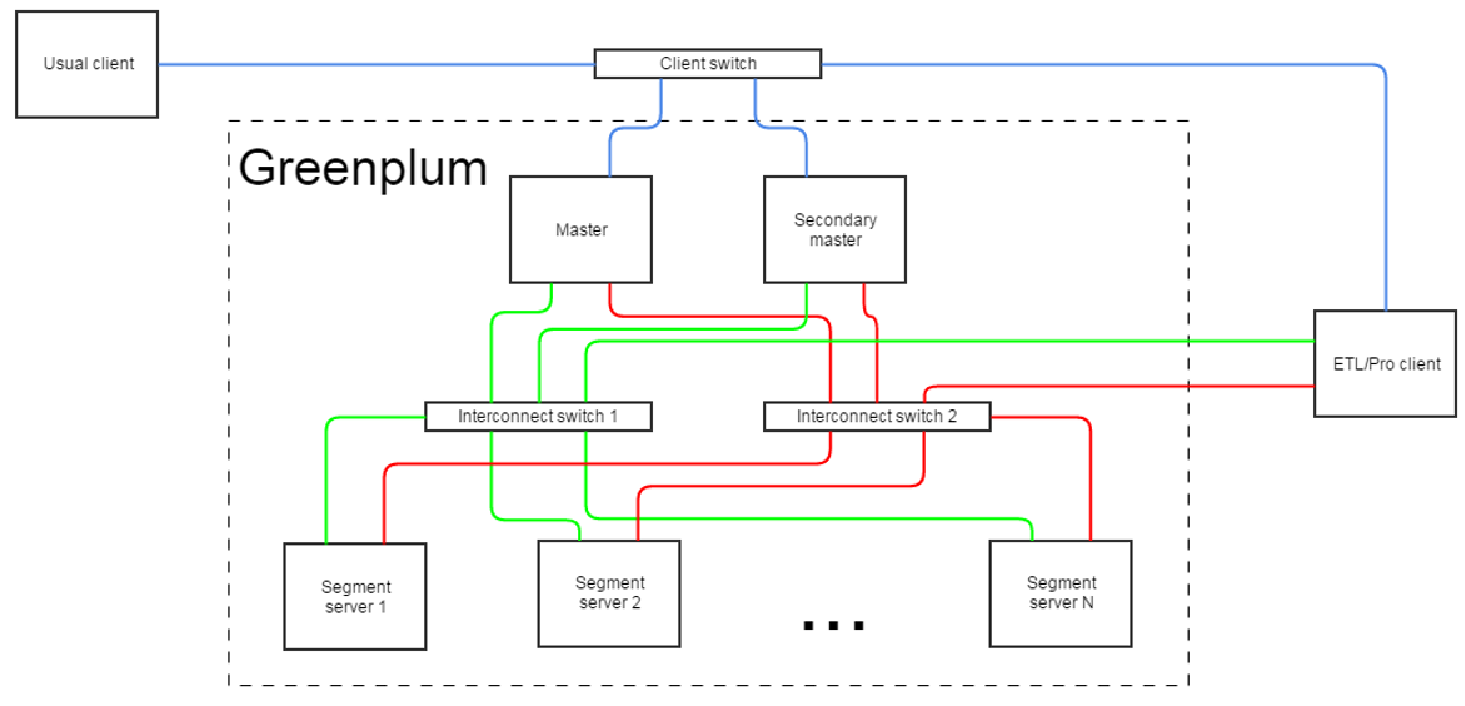
\includegraphics[width=1\textwidth]{greenplum-basic-arch.pdf}}
  \caption{Состав кластера и сетевое взаимодействие элементов. Зелёная и красная линии~--- обособленные сети interconnect, синяя линия~--- внешняя, клиентская сеть}
  \label{fig:greenplum_arch1}
\end{figure}

Использование нескольких interconnect-сетей позволяет, во-первых, повысить пропускную способность канала взаимодействия сегментов между собой, и во-вторых, обеспечить отказоустойчивость кластера (в случае отказа одной из сетей весь трафик перераспределяется между оставшимися).

При выборе числа серверов-сегментов важно правильно выбрать соотношение кластера <<число процессоров/Тб данных>> в зависимости от планируемого профиля нагрузки на БД~--- чем больше процессорных ядер приходится на единицу данных, тем быстрее кластер будет выполнять <<тяжёлые>> операции, а также работать со сжатыми таблицами.

При выборе числа сегментов в кластере (которое в общем случае к числу серверов никак не привязано) необходимо помнить следующее:

\begin{itemize}
  \item все ресурсы сервера делятся между всеми сегментами на сервере (нагрузкой зеркал, в случае если они располагаются на этих же серверах, можно условно пренебречь);
  \item каждый запрос на одном сегменте не может потреблять процессорных ресурсов больше, чем одно ядро CPU. Это означает, например, что, если кластер состоит из 32-ядерных серверов с 4-я сегментами GP на борту и используется в среднем для обработки 3-4 одновременных тяжёлых, хорошо утилизирующих CPU, запросов, <<в среднем по больнице>> CPU не будет утилизироваться оптимально. В данной ситуации лучше увеличить число сегментов на сервере до 6-8;
  \item штатный процесс бекапа и рестора данных <<из коробки>> работает только на кластерах, имеющих одинаковое число сегментов. Восстановить данные, забекапленные на кластере из 96 сегментов, в кластер из 100 сегментов без напильника будет невозможно;
\end{itemize}


\subsection{Хранение данных}
\label{subsec:greenplum_data_storage}

В Greenplum реализуется классическая схема шардирования данных. Каждая таблица представляет из себя N+1 таблиц на всех сегментах кластера, где N~--- число сегментов (+1 в этом случае — это таблица на мастере, данных в ней нет). На каждом сегменте хранится 1/N строк таблицы. Логика разбиения таблицы на сегменты задаётся ключом (полем) дистрибуции~--- таким полем, на основе данных которого любую строку можно отнести к одному из сегментов.

Ключ (поле или набор полей) дистрибуции~--- очень важное понятие в GP. Как было сказано выше, Greenplum работает со скоростью самого медленного сегмента, это означает, что любой перекос в количестве данных (как в рамках одной таблицы, так и в рамках всей базы) между сегментами ведёт к деградации производительности кластера, а также к другим проблемам. Именно поэтому следует тщательно выбирать поле для дистрибуции~--- распределение количества вхождений значений в нём должно быть как можно более равномерным. Правильно ли вы выбрали ключ дистрибуции вам подскажет служебное поле \lstinline!gp_segment_id!, существующее в каждой таблице~--- оно содержит номер сегмента, на котором хранится конкретная строка. Важный нюанс: GP не поддерживает \lstinline!UPDATE! поля, по которому распределена таблица.

Рассмотрим пример (здесь и далее в примерах кластер состоит из 96 сегментов):

\begin{lstlisting}[language=SQL,label=lst:greenplum_example1,caption=Создание распределенной таблицы]
db=# create table distrib_test_table as select generate_series(1,20) as num_field distributed by (num_field);
SELECT 20
db=# select count(1),gp_segment_id from distrib_test_table group by gp_segment_id order by gp_segment_id;
 count | gp_segment_id
-------+---------------
     1 |             4
     1 |             6
     1 |            15
     1 |            21
     1 |            23
     1 |            25
     1 |            31
     1 |            40
     1 |            42
     1 |            48
     1 |            50
     1 |            52
     1 |            65
     1 |            67
     1 |            73
     1 |            75
     1 |            77
     1 |            90
     1 |            92
     1 |            94

db=# truncate table distrib_test_table;
TRUNCATE TABLE
db=# insert into distrib_test_table values (1), (1), (1), (1), (1), (1), (1), (1), (1), (1), (1), (1), (1), (1), (1), (1), (1), (1), (1), (1);
INSERT 0 20
db=# select count(1),gp_segment_id from distrib_test_table group by gp_segment_id order by gp_segment_id;
 count | gp_segment_id
-------+---------------
    20 |            42
\end{lstlisting}

В обоих случаях распределена таблица по полю \lstinline!num_field!. В первом случае вставили в это поле 20 уникальных значений, и, как видно, GP разложил все строки на разные сегменты. Во втором случае в поле было вставлено 20 одинаковых значений, и все строки были помещены на один сегмент.

В случае, если в таблице нет подходящих полей для использования в качестве ключа дистрибуции, можно воспользоваться случайной дистрибуцией (\lstinline!DISTRIBUTED RANDOMLY!). Поле для дистрибуции можно менять в уже созданной таблице, однако после этого её необходимо перераспределить.
Именно по полю дистрибуции Greenplum совершает самые оптимальные \lstinline!JOIN!: в случае, если в обоих таблицах поля, по которым совершается \lstinline!JOIN!, являются ключами дистрибуции, \lstinline!JOIN! выполняется локально на сегменте. Если же это условие не верно, GP придётся или перераспределить обе таблицы по искомому полю, или закинуть одну из таблиц целиком на каждый сегмент (операция \lstinline!BROADCAST!) и уже затем джойнить таблицы локально на сегментах.

\begin{lstlisting}[language=SQL,label=lst:greenplum_example2,caption=JOIN по ключу дистрибуции]
db=# create table distrib_test_table as select generate_series(1,192) as num_field, generate_series(1,192) as num_field_2 distributed by (num_field);
SELECT 192
db=# create table distrib_test_table_2 as select generate_series(1,1000) as num_field, generate_series(1,1000) as num_field_2 distributed by (num_field);
SELECT 1000
db=# explain select * from distrib_test_table sq
db-# left join distrib_test_table_2 sq2
db-# on sq.num_field = sq2.num_field;
QUERY PLAN
------------------------------------------------------------------------------------------
 Gather Motion 96:1  (slice1; segments: 96)  (cost=20.37..42.90 rows=861 width=16)
   ->  Hash Left Join  (cost=20.37..42.90 rows=9 width=16)
         Hash Cond: sq.num_field = sq2.num_field
         ->  Seq Scan on distrib_test_table sq  (cost=0.00..9.61 rows=9 width=8)
         ->  Hash  (cost=9.61..9.61 rows=9 width=8)
               ->  Seq Scan on distrib_test_table_2 sq2  (cost=0.00..9.61 rows=9 width=8)
\end{lstlisting}

\begin{lstlisting}[language=SQL,label=lst:greenplum_example3,caption=JOIN не по ключу дистрибуции]
db_dev=# explain select * from distrib_test_table sq left join distrib_test_table_2 sq2
on sq.num_field_2 = sq2.num_field_2;
                                               QUERY PLAN
--------------------------------------------------------------------------------------------------------
 Gather Motion 96:1  (slice3; segments: 96)  (cost=37.59..77.34 rows=861 width=16)
   ->  Hash Left Join  (cost=37.59..77.34 rows=9 width=16)
         Hash Cond: sq.num_field_2 = sq2.num_field_2
         ->  Redistribute Motion 96:96  (slice1; segments: 96)  (cost=0.00..26.83 rows=9 width=8)
               Hash Key: sq.num_field_2
               ->  Seq Scan on distrib_test_table sq  (cost=0.00..9.61 rows=9 width=8)
         ->  Hash  (cost=26.83..26.83 rows=9 width=8)
               ->  Redistribute Motion 96:96  (slice2; segments: 96)  (cost=0.00..26.83 rows=9 width=8)
                     Hash Key: sq2.num_field_2
                     ->  Seq Scan on distrib_test_table_2 sq2  (cost=0.00..9.61 rows=9 width=8)


\end{lstlisting}


Как видно в примере <<\nameref{lst:greenplum_example3}>> в плане запроса появляются два дополнительных шага (по одному для каждой из участвующих в запросе таблиц): \lstinline!Redistribute Motion!. По сути, перед выполнением запроса GP перераспределяет обе таблицы по сегментам, используя логику поля \lstinline!num_field_2!, а не изначального ключа дистрибуции~--- поля \lstinline!num_field!.


\subsection{Взаимодействие с клиентами}

В общем случае всё взаимодействие клиентов с кластером ведётся только через мастер~--- именно он отвечает клиентам, выдаёт им результат запроса и т.д. Обычные клиенты не имеют сетевого доступа к серверам-сегментам.

Для ускорения загрузки данных в кластер используется bulk load~--- параллельная загрузка данных с/на клиент одновременно с нескольких сегментов. Bulk load возможен только с клиентов, имеющих доступ в интерконнекты. Обычно в роли таких клиентов выступают ETL-сервера и другие системы, которым необходима загрузка большого объёма данных (на рис~\ref{fig:greenplum1} они обозначены как ETL/Pro client).

Для параллельной загрузки данных на сегменты используется утилита \lstinline!gpfdist!. По сути, утилита поднимает на удалённом сервере web-сервер, который предоставляет доступ по протоколам gpfdist и http к указанной папке. После запуска директория и все файлы в ней становятся доступны обычным \lstinline!wget!. Создадим для примера файл в директории, обслуживаемой \lstinline!gpfdist!, и обратимся к нему как к обычной таблице.

\begin{lstlisting}[language=SQL,label=lst:greenplum_example4,caption=Пример с gpfdist]
# На ETL-сервере:
bash# for i in {1..1000}; do echo "$i,$(cat /dev/urandom | tr -dc 'a-zA-Z0-9' | fold -w 8 | head -n 1)"; done > /tmp/work/gpfdist_home/test_table.csv

# Теперь создаим внешнюю таблицу и прочитаем данные из файла
# В Greenplum DB:
db=# create external table ext_test_table
db-# (id integer, rand varchar(8))
db-# location ('gpfdist://etl_hostname:8081/test_table.csv')
db-# format 'TEXT' (delimiter ',' NULL ' ');
CREATE EXTERNAL TABLE
db_dev=# select * from ext_test_table limit 100;
NOTICE:  External scan from gpfdist(s) server will utilize 64 out of 96 segment databases
 id  |   rand
-----+----------
   1 | UWlonJHO
   2 | HTyJNA41
   3 | CBP1QSn1
   4 | 0K9y51a3
...
\end{lstlisting}

Также, но с немного другим синтаксисом, создаются внешние web-таблицы. Их особенность заключается в том, что они ссылаются на http протокол, и могут работать с данными, предоставляемыми сторонними web-серверами (apache, nginx и другие).

В Greenplum также существует возможность создавать внешние таблицы на данные, лежащие на распределённой файловой системе Hadoop (hdfs)~--- за это в GP ответственна отдельная компонента \lstinline!gphdfs!. Для обеспечения её работы на каждый сервер, входящий в состав кластера GP, необходимо установить библиотеки Hadoop и прописать к ним путь в одной из системных переменных базы. Создание внешней таблицы, обращающейся к данным на hdfs, будет выглядеть примерно так:

\begin{lstlisting}[language=SQL,label=lst:greenplum_example5,caption=Пример с gphdfs]
db=# create external table hdfs_test_table
db=# (id int, rand text)
db=# location('gphdfs://hadoop_name_node:8020/tmp/test_file.csv')
db=# format 'TEXT' (delimiter ',');
\end{lstlisting}

где \lstinline!hadoop_name_node!~--- адрес хоста неймноды, \lstinline!/tmp/test_file.csv!~--- путь до искомого файла на hdfs.

При обращении к такой таблице Greenplum выясняет у неймноды Hadoop расположение нужных блоков данных на датанодах, к которым затем обращается с серверов-сегментов параллельно. Естественно, все ноды кластера Hadoop должны быть в сетях интерконнекта кластера Greenplum. Такая схема работы позволяет достичь значительного прироста скорости даже по сравнению с \lstinline!gpfdist!. Что интересно, логика выбора сегментов для чтения данных с датанод hdfs является весьма нетривиальной. Например, GP может начать тянуть данные со всех датанод только двумя сегмент-серверами, причём при повторном аналогичном запросе схема взаимодействия может поменяться.

Также есть тип внешних таблиц, которые ссылаются на файлы на сегмент-серверах или файл на мастере, а также на результат выполнения команды на сегмент-серверах или на мастере. К слову сказать, старый добрый \lstinline!COPY FROM! никуда не делся и также может использоваться, однако по сравнению с описанным выше работает он медленней.


\subsection{Надёжность и резервирование}

\subsubsection{Резервирование мастера}

Как было сказано ранее, в кластере GP используется полное резервирование мастера с помощью механизма репликации транзакционных логов, контролируемого специальным агентом (\lstinline!gpsyncagent!). При этом автоматическое переключение роли мастера на резервный инстанс не поддерживается. Для переключения на резервный мастер необходимо:

\begin{itemize}
  \item убедиться, что основной мастер остановлен (процесс убит и в рабочей директории инстанса мастера отсутствует файл postmaster.pid);
  \item на сервере резервного мастера выполнить команду \lstinline!gpactivatestandby -d /master_instance_directory!;
  \item переключить виртуальный ip-адрес на сервер нового мастера (механизм виртуального ip в Greenplum отсутствует, необходимо использовать сторонние инструменты);
\end{itemize}

Как видно, переключение выполняется совсем не сложно и при принятии определённых рисков может быть автоматизировано.


\subsubsection{Резервирование сегментов}

Схема резервирования сегментов похожа на таковую для мастера, отличия совсем небольшие. В случае падения одного из сегментов (инстанс PostgreSQL перестаёт отвечать мастеру в течении таймаута) сегмент помечается как сбойный, и вместо него автоматически запускается его зеркало (по сути, абсолютно аналогичный инстанс PostgreSQL). Репликация данных сегмента в его зеркало происходит на основе кастомной синхронной репликации на уровне файлов.

Cтоит отметить, что довольно важное место в процессе планирования архитектуры кластера GP занимает вопрос расположения зеркал сегментов на серверах, благо GP даёт полную свободу в вопросе выбора мест расположения сегментов и их зеркал: с помощью специальной карты расположения сегментов их можно разместить на разных серверах, в разных директориях и заставить использовать разные порты. Рассмотрим два варианта:

\begin{figure}[ht!]
  \center{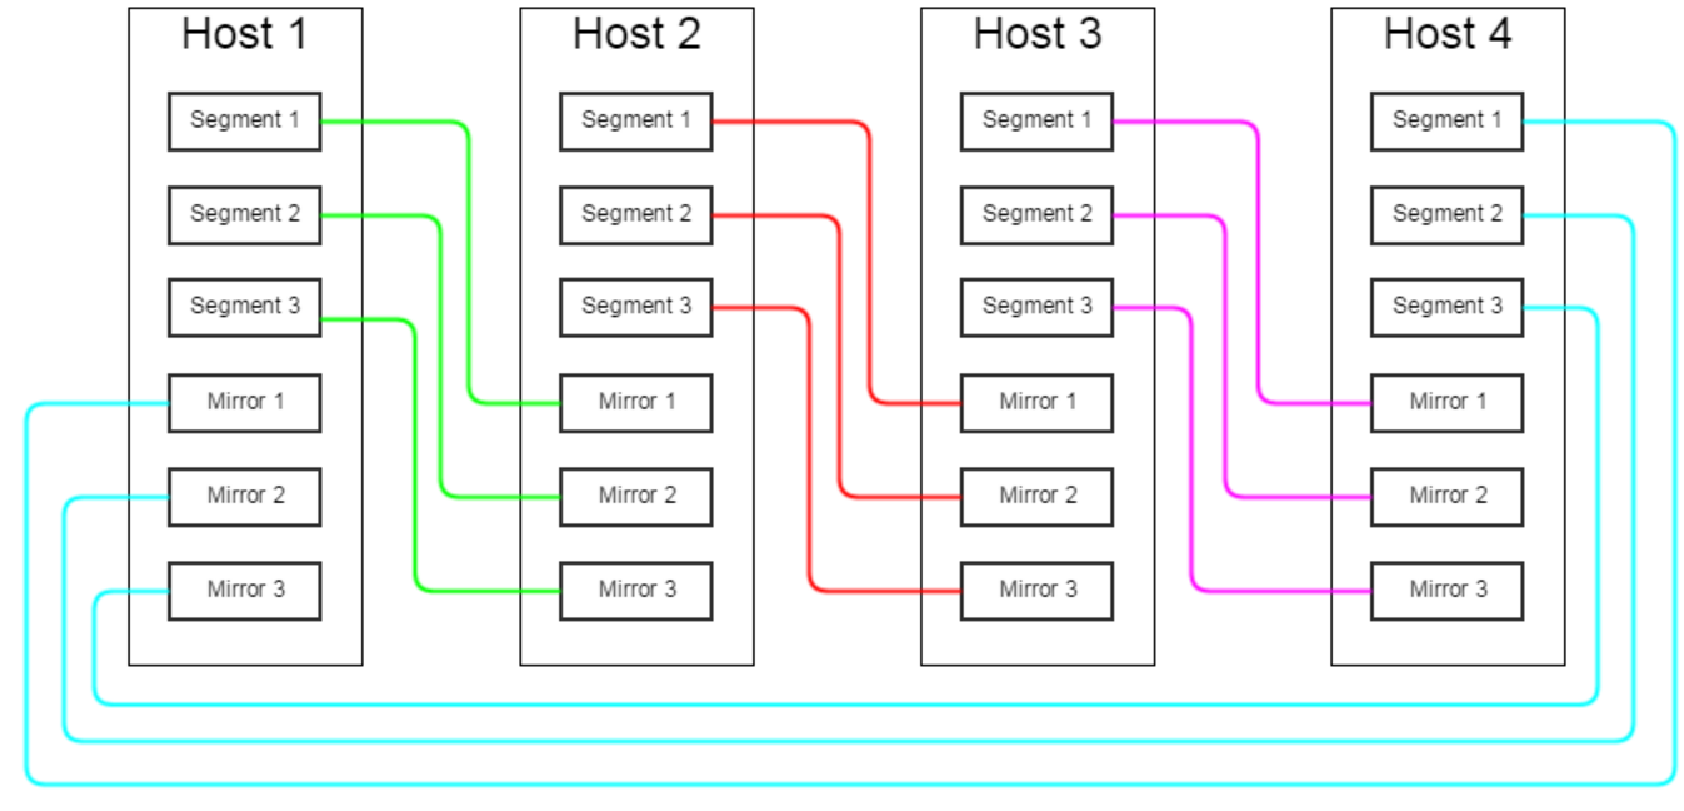
\includegraphics[width=1\textwidth]{greenplum-reserving-one.pdf}}
  \caption{Все зеркала сегментов, располагающихся на хосте N, находятся на хосте N+1}
  \label{fig:greenplum_reserve_one}
\end{figure}

При использовании схемы~\ref{fig:greenplum_reserve_one} при отказе одного из серверов на сервере-соседе оказывается в два раза больше работающих сегментов. Как было сказано выше, производительность кластера равняется производительности самого медленного из сегментов, а значит, в случае отказа одного сервера производительность базы снижается минимум вдвое. Однако, такая схема имеет и положительные стороны: при работе с отказавшим сервером уязвимым местом кластера становится только один сервер~--- тот самый, куда переехали сегменты.

\begin{figure}[ht!]
  \center{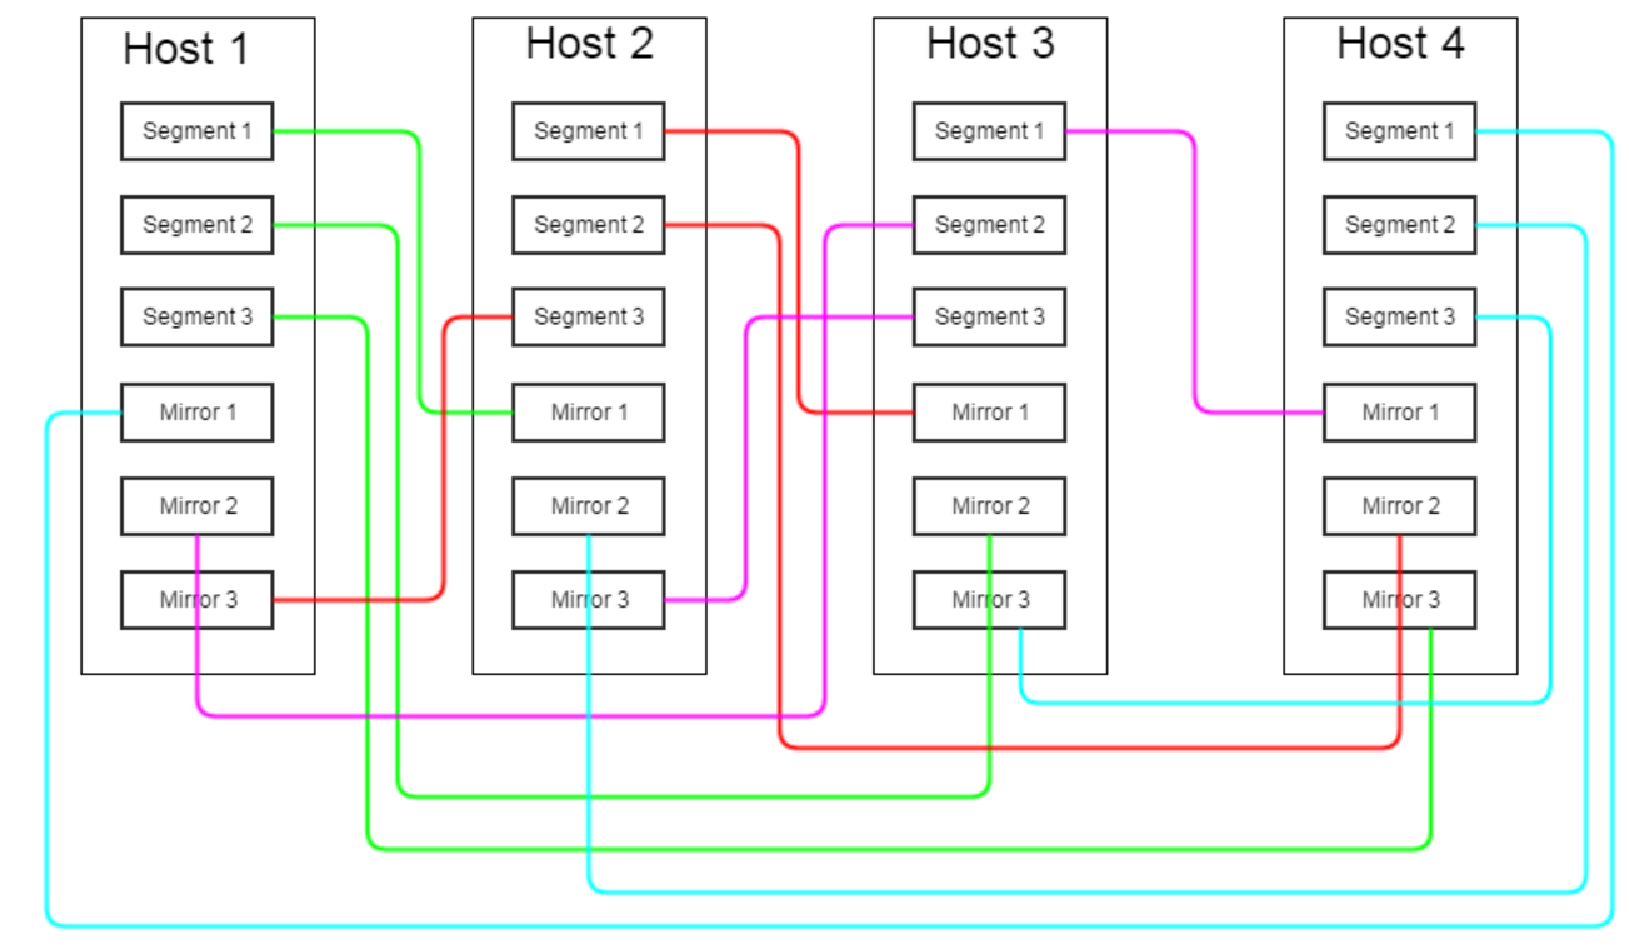
\includegraphics[width=1\textwidth]{greenplum-reserving-two.pdf}}
  \caption{Все зеркала сегментов, располагающихся на хосте N, равномерно <<мажутся>> на сервера N+1, N+2 ... N+M, где M – число сегментов на сервере}
  \label{fig:greenplum_reserve_two}
\end{figure}

При использовании схемы~\ref{fig:greenplum_reserve_two} в случае отказа сервера возросшая нагрузка равномерно распределяется между несколькими серверами, не сильно влияя на общую производительность кластера. Однако, существенно повышается риск выхода из строя всего кластера~--- достаточно выйти из строя одному из M серверов, соседствующих с вышедшим из строя изначально.

Истина, как это часто бывает, где-то посередине~--- можно расположить по несколько зеркал сегментов одного сервера на нескольких других серверах, можно объединять сервера в группы отказоустойчивости, и так далее. Оптимальную конфигурацию зеркал следует подбирать исходя из конкретных аппаратных данных кластера, критичности простоя и так далее.

Также в механизме резервирования сегментов есть ещё один нюанс, влияющий на производительность кластера. В случае выхода из строя зеркала одного из сегментов последний переходит в режим \lstinline!change tracking!~--- сегмент логирует все изменения, чтобы затем при восстановлении упавшего зеркала применить их к нему, и получить свежую, консистентную копию данных. Другими словами, при падении зеркала нагрузка, создаваемая на дисковую подсистему сервера сегментом, оставшимся без зеркала, существенно возрастает.

При устранении причины отказа сегмента (аппаратные проблемы, кончившееся место на устройстве хранения и прочее) его необходимо вернуть в работу вручную, с помощью специальной утилиты \lstinline!gprecoverseg! (даунтайм СУБД не требуется). По факту эта утилита скопирует скопившиеся на сегменте WA-логи на зеркало и поднимет упавший сегмент/зеркало. В случае, если речь идёт о primary-сегменте, изначально он включится в работу как зеркало для своего зеркала, ставшего primary (зеркало и основной сегмент будут работать поменявшись ролями). Для того, чтобы вернуть всё на круги своя, потребуется процедура ребаланса~--- смены ролей. Такая процедура также не требует даунтайма СУБД, однако на время ребаланса все сессии в БД подвиснут.

В случае, если повреждения упавшего сегмента настолько серьёзны, что простым копированием данных из WA-логов не обойтись, есть возможность использовать полное восстановление упавшего сегмента~--- в таком случае, по факту, инстанс PostgreSQL будет создан заново, однако за счёт того, что восстановление будет не инкрементальным, процесс восстановления может занять продолжительное время.


\subsection{Производительность}

Оценка производительности кластера Greenplum – понятие довольно растяжимое. Исходные данные: кластер из 24 сегмент-серверов, каждый сервер~--- 192 Гб памяти, 40 ядер. Число primary-сегментов в кластере: 96. В первом примере мы создаём таблицу с 4-я полями + первичный ключ по одному из полей. Затем мы наполняем таблицу данными (10 000 000 строк) и пробуем выполнить простой \lstinline!SELECT! с несколькими условиями.

\begin{lstlisting}[language=SQL,label=lst:greenplum_example5,caption=SELECT с условиями]
db=# CREATE TABLE test3
db-# (id bigint NOT NULL,
db(# profile bigint NOT NULL,
db(# status integer NOT NULL,
db(# switch_date timestamp without time zone NOT NULL,
db(# CONSTRAINT test3_id_pkey PRIMARY KEY (id) )
db-# distributed by (id);
NOTICE:  CREATE TABLE / PRIMARY KEY will create implicit index "test3_pkey" for table "test3"
CREATE TABLE

db=# insert into test3 (id , profile,status, switch_date) select a, round(random()*100000), round(random()*4), now() - '1 year'::interval * round(random() * 40) from generate_series(1,10000000) a;
INSERT 0 10000000

db=# explain analyze  select  profile, count(status) from test3
db=#                         where status<>2
db=#                         and switch_date between '1970-01-01' and '2015-01-01'  group by profile;

Gather Motion 96:1 (slice2; segments: 96) (cost=2092.80..2092.93 rows=10 width=16)
Rows out: 100001 rows at destination with 141 ms to first row, 169 ms to end, start offset by 0.778 ms.
-> HashAggregate (cost=2092.80..2092.93 rows=1 width=16)
   Group By: test3.profile
   Rows out: Avg 1041.7 rows x 96 workers. Max 1061 rows (seg20) with 141 ms to end, start offset by 2.281 ms.
   Executor memory: 4233K bytes avg, 4233K bytes max (seg0).
   -> Redistribute Motion 96:96 (slice1; segments: 96) (cost=2092.45..2092.65 rows=1 width=16)
      Hash Key: test3.profile
      Rows out: Avg 53770.2 rows x 96 workers at destination. Max 54896 rows (seg20) with 71 ms to first row, 117 ms to end, start offset by 5.205 ms.
      -> HashAggregate (cost=2092.45..2092.45 rows=1 width=16)
      Group By: test3.profile
      Rows out: Avg 53770.2 rows x 96 workers. Max 54020 rows (seg69) with 71 ms to first row, 90 ms to end, start offset by 7.014 ms.
      Executor memory: 7882K bytes avg, 7882K bytes max (seg0).
      -> Seq Scan on test3 (cost=0.00..2087.04 rows=12 width=12)
         Filter: status <> 2 AND switch_date >= '1970-01-01 00:00:00'::timestamp without time zone AND switch_date <= '2015-01-01 00:00:00'::timestamp without time zone
         Rows out: Avg 77155.1 rows x 96 workers. Max 77743 rows (seg26) with 0.092 ms to first row, 31 ms to end, start offset by 7.881 ms.
Slice statistics:
(slice0) Executor memory: 364K bytes.
(slice1) Executor memory: 9675K bytes avg x 96 workers, 9675K bytes max (seg0).
(slice2) Executor memory: 4526K bytes avg x 96 workers, 4526K bytes max (seg0).
Statement statistics:
Memory used: 128000K bytes
Total runtime: 175.859 ms
\end{lstlisting}

Как видно, время выполнения запроса составило 175 мс. Теперь попробуем пример с джойном по ключу дистрибуции одной таблицы и по обычному полю другой таблицы.

\begin{lstlisting}[language=SQL,label=lst:greenplum_example6,caption=JOIN по ключу дистрибуции одной таблицы и по обычному полю другой]
db=# create table test3_1 (id bigint NOT NULL, name text, CONSTRAINT test3_1_id_pkey PRIMARY KEY (id)) distributed by (id);
NOTICE:  CREATE TABLE / PRIMARY KEY will create implicit index "test3_1_pkey" for table "test3_1"
CREATE TABLE
db=# insert into test3_1 (id , name) select a, md5(random()::text) from generate_series(1,100000) a;
INSERT 0 100000
db=# explain analyze select test3.*,test3_1.name from test3 join test3_1 on test3.profile=test3_1.id;

-> Hash Join (cost=34.52..5099.48 rows=1128 width=60)
   Hash Cond: test3.profile = test3_1.id
   Rows out: Avg 104166.2 rows x 96 workers. Max 106093 rows (seg20) with 7.644 ms to first row, 103 ms to end, start offset by 223 ms.
   Executor memory: 74K bytes avg, 75K bytes max (seg20).
   Work_mem used: 74K bytes avg, 75K bytes max (seg20). Workfile: (0 spilling, 0 reused)
   (seg20) Hash chain length 1.0 avg, 1 max, using 1061 of 262151 buckets.
   -> Redistribute Motion 96:96 (slice1; segments: 96) (cost=0.00..3440.64 rows=1128 width=28)
      Hash Key: test3.profile
      Rows out: Avg 104166.7 rows x 96 workers at destination. Max 106093 rows (seg20) with 3.160 ms to first row, 44 ms to end, start offset by 228 ms.
      -> Seq Scan on test3 (cost=0.00..1274.88 rows=1128 width=28)
      Rows out: Avg 104166.7 rows x 96 workers. Max 104209 rows (seg66) with 0.165 ms to first row, 16 ms to end, start offset by 228 ms.
   -> Hash (cost=17.01..17.01 rows=15 width=40)
      Rows in: Avg 1041.7 rows x 96 workers. Max 1061 rows (seg20) with 1.059 ms to end, start offset by 227 ms.
      -> Seq Scan on test3_1 (cost=0.00..17.01 rows=15 width=40)
         Rows out: Avg 1041.7 rows x 96 workers. Max 1061 rows (seg20) with 0.126 ms to first row, 0.498 ms to end, start offset by 227 ms.
Slice statistics:
(slice0) Executor memory: 364K bytes.
(slice1) Executor memory: 1805K bytes avg x 96 workers, 1805K bytes max (seg0).
(slice2) Executor memory: 4710K bytes avg x 96 workers, 4710K bytes max (seg0). Work_mem: 75K bytes max.
Statement statistics:
Memory used: 128000K bytes
Total runtime: 4526.065 ms
\end{lstlisting}

Время выполнения запроса составило 4.6 секунды. Много это или мало для такого объёма данных~--- вопрос спорный и лежащий вне этой книги.



\subsection{Расширение кластера}

В жизненном цикле распределённой аналитической БД рано или поздно возникает ситуация, когда объём доступного дискового пространства уже не может вместить всех необходимых данных, а добавление устройств хранения в имеющиеся сервера либо невозможна, либо слишком дорога и сложна (потребуется, как минимум, расширение существующих разделов). Кроме того, добавление одних лишь дисковых мощностей негативно скажется на соотношении <<число процессоров/Тб данных>>, о котором мы говорили в <<\ref{subsec:greenplum_data_storage}~\nameref{subsec:greenplum_data_storage}>>. Говоря простым языком, в кластер рано или поздно понадобится вводить новые сервера. Greenplum позволяет добавлять как новые сервера, так и новые сегменты практически без простоя СУБД. Последовательность этого действа примерно такая:

\begin{itemize}
  \item разработать карту сегментов, согласно которой GP будет размещать новые сегменты и зеркала на новых серверах;
  \item сделать бекап необходимых критичных данных (как минимум всех метаданных);
  \item установить ПО СУБД на новые сервера;
  \item остановить СУБД (следующий пункт выполняется в даунтайм);
  \item инициализировать новые сегменты утилитой \lstinline!gpexpand! (занимает от 5 до 10 минут);
  \item поднять СУБД (даунтайм окончен);
  \item перераспределить (redistribute) все таблицы;
  \item собрать статистику (analyze) по всем таблицам;
\end{itemize}

Как видно, хотя процедура расширения и продолжительна, полная недоступность БД при правильных действиях администратора не превысит 20-30 минут.


\subsection{Особенности эксплуатации}

Как обычно, практика вносит в красивую теорию свои коррективы. Поделюсь некоторыми нюансами эксплуатации, выявленными нами за долгое время использования GP. Сразу оговорюсь, что стандартные нюансы PostgreSQL (необходимость \lstinline!VACUUM!, особенности репликации) в этот перечень не попали.

\begin{itemize}
  \item Автоматический failover не даёт 100\% гарантии переключения на зеркало. Увы, но это так, особенно под нагрузкой, есть риск зависания процессов базы при попытке переключения на зеркало. Частично проблему решает уменьшение таймаута ответа от сегментов до нескольких минут, однако даже в таком случае риск остаётся. Как частное решение проблемы зависания при переключении можно использовать ручное убийство зависшего сегмента или перезагрузку базы;
  \item Greenplum и OLTP несовместимы. GP~--- аналитическая БД, предназначенная для небольшого числа одновременных запросов, выполняющих тяжёлые операции над большим объёмом данных. Большое число (более 600 queries per second) лёгких запросов/транзакций, выполняющих одну операцию, негативно сказывается на производительности базы из-за её распределённой архитектуры~--- каждая транзакция на мастере порождает N транзакций на сегментах. Хорошей практикой является агрегация большого числа \lstinline!UPDATE/INSERT! в батчи;
  \item Отсутствие механизма инкрементального бекапа;
  \item Свой синтаксис. Несмотря на то, что для клиента Greenplum по сути является PostgreSQL DB, небольшие различия в синтаксисе SQL заставляют использовать стандартный клиентский PostgreSQL-софт с большой осторожностью;
  \item Отсутствие возможности пометить сегменты как <<архивные>>. Частично этот недостаток можно решить путём использования архивных партиций, находящихся на медленном дешевом tablespace, а также c помощью появившейся в последней на момент написания статьи версии GP 4.3.6.0 возможности располагать партиции таблицы во внешних источниках (например, внешних таблицах \lstinline!gphdfs!, лежащих в кластере Hadoop);
  \item Greenplum использует PostgreSQL версии 8.3.23, а значит о многих современных плюшках этой замечательной БД придётся забыть;
\end{itemize}


\subsection{Заключение}

Greenplum~--- мощный и гибкий инструмент для аналитической обработки больших объёмов данных. Он требует к себе немного другого подхода, чем остальные enterprise-level решения для Data Warehouse (<<напильник>>~--- любимый инструмент администратора GP). Однако при достаточно низком пороге вхождения и большой унифицированности с PostgreSQL Greenplum является сильным игроком на поле Data Warehouse DB.




\section{Заключение}

В данной главе рассмотрены лишь базовые настройки кластеров БД. Про кластеры PostgreSQL потребуется написать отдельную книгу, чтобы рассмотреть все шаги с установкой, настройкой и работой кластеров. Надеюсь, что несмотря на это, информация будет полезна многим читателям.
